%\documentclass{article}
%\usepackage[utf8]{inputenc}
%\usepackage{amsmath}
%\usepackage{amsthm}
%\usepackage{amssymb}
%\usepackage{enumitem}
%\usepackage[left=2.5cm,right=2.5cm,top=2.25cm,bottom=2.25cm]{geometry}
%\usepackage{multirow}
%
%\title{LINMA2471 -- Optimization models ans methods II \\ Notes from the $6^\mathrm{th}$ lecture}
%\author{Antoine Aspeel \and Pierre-Paul Mouchet \and Guillaume Olikier}
%\date{October 21, 2015}
%
%% Definitions and propositions
%\newtheorem{theorem}{Theorem}
%\newtheorem{prop}[theorem]{Proposition}
%\newtheorem{lemma}[theorem]{Lemma}
%\newtheorem{coro}[theorem]{Corollary}
%\theoremstyle{definition}
%\newtheorem{definition}{Definition}
%\newtheorem{ex}{Example}
%
%% Shortcuts

%
%
%
%\begin{document}
%
%\maketitle





\section{Gradient method for unconstrained problems}

\subsection{Gradient method for functions of $C_L^{1,1}$}

In the previous section, we studied the gradient method for the general problem.
\begin{equation*}
\min_{x \in \mathbb{R}^n} f(x)
\end{equation*}
where $f \in C_L^{1,1}(\mathbb{R}^n)$. We proved that $\frac{1}{L}$ was actually the best step length choice and that it guaranteed
\begin{equation}
\min_{0 \le i \le N} \vnorm{\nabla f(x_i)} \le \sqrt{\frac{2L(f(x_0)-f(x^*))}{N+1}} .
\label{MinGrad}
\end{equation}
Observe that this inequality
\begin{itemize}
\item is scaling independent,
\item doesn't say anything about the values of $f$.
\end{itemize}
One can show that this inequality is not improvable. \\

Let us recall the way we obtained the above inequality.

\begin{lemma}[Quadratic bounds in $C_L^{1,1}$]
The following conditions are equivalent :
\begin{enumerate}% [label=(\alph*)]
\item $f \in C_L^{1,1}(D)$,
\item $f \in C^1(D)$ and $|f(y) - T_x^1(y)| \le \frac{L}{2}\vnorm{x-y}^2$ $\forall x,y \in D$.
\end{enumerate}
\label{qbCL}
\end{lemma}
\begin{proof}
See the fourth exercises session.
\end{proof}

From this lemma, we concluded that $\frac{1}{L}$ is the optimal step length.

\begin{theorem}[Decrease guarantee]
Let $f \in C_L^{1,1}$. Denote $x^+ = x - \frac{1}{L}\nabla f(x)$ the next iterate. Then
\begin{equation*}
f(x) - f(x^+) \ge \frac{{\vnorm{\nabla f(x)}}^2}{2L}.
\end{equation*}
\label{DecreaseGuar}
\end{theorem}
\begin{proof}
Use the upper bound of lemma \ref{qbCL} with $y = x^+$.
\end{proof}
\noindent Actually there exist a family of functions which can be as closed of this bound as you want. \\

Finally theorem \ref{DecreaseGuar} leads to the inequality \eqref{MinGrad}.

\subsection{Gradient method for functions of $F_L^{1,1}$}

Let us now consider the same problem with the additional assumption $f \in F_L^{1,1}(\mathbb{R}^n)$. Lemma \ref{qbCL} can be improved as follows.

\begin{lemma}[Quadratic bounds in $F_L^{1,1}$]
The following conditions are equivalent :
\begin{enumerate}%[label=(\alph*)]
\item $f \in F_L^{1,1}(D)$,
\item $f \in C^1(D)$ and $T_y^1(x) \le f(x) \le  T_y^1(x) + \frac{L}{2}\vnorm{x-y}^2$ for all $x,y \in D$.
\end{enumerate}
\label{qbFL}
\end{lemma}
\begin{proof}
See the fourth exercises session.
\end{proof}

\begin{lemma}
Let $f \in C_L^{1,1}$. For any optimal solution $x^*$ and any $x$,
\begin{equation*}
\frac{{\vnorm{\nabla f(x)}}^2}{2L} \le f(x) - f(x^*) \le \frac{L}{2} {\vnorm{x-x^*}}^2 .
\end{equation*}
\end{lemma}
\begin{proof}
The first inequality follows from theorem \ref{DecreaseGuar} since $f(x^+) \ge f(x^*)$. The second inequality follows from lemma \ref{qbCL} applied with $x = x^*$. Indeed since $f \in C^1$ and $x^*$ is a local extremum, we have $\nabla f(x^*) = 0$.
\end{proof}

\begin{theorem}[Convergence of $\frac{1}{L}$-gradient method for $F_L^{1,1}$]
Let $f \in F_L^{1,1}$. For any iterate $x_N$ and any $x_0$,
\begin{equation*}
f(x_N) - f(x^*) \le \frac{L}{2N} \vnorm{x_0-x^*}^2 .
\end{equation*}
\end{theorem}
\begin{proof}
We start from theorem \ref{DecreaseGuar}:
\begin{equation*}
f(x^+) \le f(x) - \frac{{\vnorm{\nabla f(x)}}^2}{2L} .
\end{equation*}
Since $f \in C^1$ and $f$ is convex, we have
\begin{equation*}
f(x^*) \ge f(x) + \nabla f(x)^T(x^*-x),
\end{equation*}
right-hand side being tangent equation around $x$. Combining these two inequalities yields
\begin{equation*}
f(x^+) \le f(x^*) + \nabla f(x)^T(x-x^*) - \frac{1}{2L} {\vnorm{\nabla f(x)}}^2 .
\end{equation*}
Now, observe that\footnote{Apply $\vnorm{a-b}^2 = \vnorm{a}^2 - 2a^Tb + \vnorm{b}^2$ to $a = x-x^*$ and $b = \frac{1}{L}\nabla f(x)$. Ok, it's a trick.}
\begin{equation*}
\nabla f(x)^T(x-x^*) - \frac{1}{2L}{\vnorm{\nabla f(x)}}^2 = \frac{L}{2} \left( \vnorm{x-x^*}^2 - \vnorm{x-x^*-\frac{1}{L}\nabla f(x)}^2 \right) .
\end{equation*}
Noting that $x-\frac{1}{L}\nabla f(x) = x^+$, we obtain
\begin{equation*}
f(x^+) - f(x^*) \le \frac{L}{2} \left( \vnorm{x-x^*}^2 - \vnorm{x^+-x^*}^2 \right) .
\end{equation*}
So given $N \in \mathbb{N}$, we have for all $i \in \{0,...,N-1\}$
\begin{equation*}
f(x_{i+1}) - f(x^*) \le \frac{L}{2} \left( \vnorm{x_i-x^*}^2 - \vnorm{x_{i+1}-x^*}^2 \right) .
\end{equation*}
Summing those $N$ inequalities yields
\begin{align*}
\sum_{i=0}^{N-1}f(x_{i+1}) - N f(x^*) &\le \frac{L}{2} \sum_{i=0}^{N-1}\left( \vnorm{x_i-x^*}^2 - \vnorm{x_{i+1}-x^*}^2 \right) \\
&= \frac{L}{2} \left( \vnorm{x_0-x^*}^2 - \vnorm{x_N-x^*}^2 \right) \\
&\le \frac{L}{2} \vnorm{x_0-x^*}^2 .
\end{align*}
Notice now that $f(x_N) \le f(x_i)$ for all $i \in \{0,...,N-1\}$ so that
\begin{equation*}
 N f(x_N) \le \sum_{i=1}^Nf(x_i) .
\end{equation*}
Using this in the last inequality, we finally get
\begin{equation*}
f(x_{N}) - f(x^*) \le  \frac{L}{2N} \vnorm{x_0-x^*}^2 . \qedhere
\end{equation*}
\end{proof}

Among all methods with
\begin{equation*}
x_k \in \myspan\{x_0, \nabla f(x_0), ..., \nabla f(x_{N-1})\},
\end{equation*}
none of them can guarantee better than
\begin{equation*}
f(x_N) - f(x^*) \le \frac{3}{32}L \frac{{\vnorm{x_0-x^*}}^2}{(N+1)^2}
\end{equation*}
for dimension greater or equal to $2N+1$.

\section{Gradient method for constrained problems}

We now add constraints. We consider problems of the following form:
\begin{equation*}
\min_{x \in C} f(x) \qquad \text{with} \quad f \in C_L^{1,1}(C)
\end{equation*}
and
\begin{equation*}
\min_{x \in C} f(x) \qquad \text{with} \quad f \in F_L^{1,1}(C) .
\end{equation*}
We assume $C \subseteq \mathbb{R}^n$ is a convex and closed set. This implies that the orthogonal projection on $C$
\begin{equation*}
P_C : \mathbb{R}^n \to C : x \mapsto P_C(x)
\end{equation*}
is well defined and unique.\\

\begin{definition}
Let $\mathcal{C}$ be a closed convex set and f a differentiable function ($f \in C_L^{1,1}(C)$), we say that $x^*$ is a \textbf{stationary point} of the problem $\min\limits_{x \in C} f(x)$ if and only if
\begin{equation*}
\langle \nabla f(x^*), x-x^* \rangle \ \geq\ 0 \ \ \ \ \forall x \in C
\end{equation*}
\end{definition}
This definition can be intuitively interpreted as follows: adding $f(x^*)$ on both sides brings up the first-order Taylor expansion of $f$ around $x^*$, which is closed to $f(x)$. So this definition essentially means $f(x) \ge f(x^*)$.\\
In another interpretation, that means that all possible errors $x-x^*$ are in opposite direction with $-\nabla f$. A schema of the situation is shown on figure \ref{tik1}.
\begin{figure}[H]
\centering
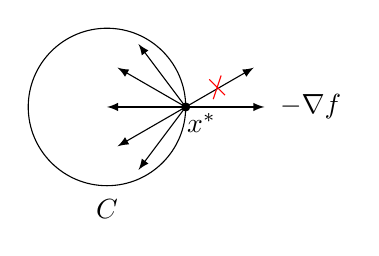
\begin{tikzpicture}
\draw (0,0) circle (1);
\draw[fill = black] (1,0) circle (0.05);
\draw (0,-1.3) node{$C$};
\draw (1.2,-0.2) node{$x^*$};
\draw[>=latex,->] (1,0) -- (2,0) node{$\ \ \ \ \ \ \ \ \ \ -\nabla f$};
\draw[>=latex,->] (1,0) -- (1.866025403784439,0.5);
\draw[>=latex,->] (1,0) -- (0,0);
\draw[>=latex,->] (1,0) -- (0.133974596215561,0.5);
\draw[>=latex,->] (1,0) -- (0.133974596215561,-0.5);
\draw[>=latex,->] (1,0) -- (0.4,0.8);
\draw[>=latex,->] (1,0) -- (0.4,-0.8);
\draw[red] (1.5,0.15) -- (1.3,0.35);
\draw[red] (1.35,0.1) -- (1.45,0.4);
\end{tikzpicture}
\caption{Example of a stationnary point $x^*$.}
\label {tik1}
\end{figure}

\begin{example}
\begin{leftbar}
 $C = \{x \in \mathbb{R}^n: x_i \ge 0\}$ (nonnegative orthant)
\begin{align*}
&x^* \; \text{stationnary iff} \; \sum_i \left[\nabla f(x^*)\right]_i \left[x_i - x_i^*\right] \ge 0\ \ \ \forall x\ge 0\\
&x^* \; \text{stationnary iff either} \; [\nabla f(x^*)]_i=0\\ 
&\phantom{x^* \; \text{stationnary iff eith}}\text{or} \; [\nabla f(x^*)]_i>0 \; \text{and} \; x_i^*=0 \; \forall \; i
\end{align*}
Indeed, as $\sum_i [x_i - x_i^*] \ge 0$ for all $x\ge0$,  $[\nabla f(x^*)]_i$ must be $\ge 0$.
If not, we could choose a very large $x_i$ for this component and have a negative sum.
\end{leftbar}
\end{example}

\begin{example}
\begin{leftbar}
It also works easily for $C = \{x|\sum_{i}x_i=1\}$ which is a kind of budget constraint. In that case, it is possible to show that $[\nabla f(x^*)]_i = \lambda \; \forall i$. That means that all the gradient components are equal to each other, or economically speaking that the marginal costs are equal to each other. At the optimum, the marginal cost is equal for each component, it does not matter which one you lower.
\end{leftbar}
\end{example}

\begin{example}
\begin{leftbar}
(not treated) The Euclidian bowl.
\end{leftbar}
\end{example}


Note that if $x^* \in \myint\, C$, then necessarily $\nabla f(x^*) = 0$.
Indeed, if $\nabla f(x^*) \neq 0$ and $x^* \in \myint\, C$, we can choose $x$ such that $\nabla f(x^*)$ and $x-x^*$ are of opposite directions. Consequently, their scalar product is negative which contradicts the definition of $x^*$. This implies that $\nabla f(x^*) = 0$.

\begin{theorem}
Under the above assumptions, if $x^*$ is a local minimum, then $x^*$ is stationary.
\end{theorem}

\begin{theorem}
When $f$ is convex, stationary implies optimality.
\end{theorem}


\subsection{Projected gradient method}
Let us now present the gradient method for constrained problems. The principle is the following:
\begin{enumerate}
\item at each step, minimize the quadratic upper bound on set $C$,
\item which is equivalent to projecting the true minimum of the quadratic upper bound on set $C$.
\end{enumerate}
Let us show this equivalence. Statements mean
\begin{enumerate}
\item choose $x^+$ minimizing $f(x) + \nabla f(x)^T(x^+-x) + \frac{L}{2}{\vnorm{x-x^+}}^2$ over $C$, where we can ignore the constant term $f(x)$ in the minimization problem,
\item choose $x^+$ minimizing ${\vnorm{x^+ - (x - \frac{1}{L}\nabla f(x))}^2}$ over $C$. Notice that we can develop
\begin{equation*}
\begin{array}{rcl}
\vnorm{x^+ - (x - \frac{1}{L}\nabla f(x))}^2 & = & \vnorm{(x^+ - x) + \frac{1}{L}\nabla f(x))}^2 \\
& = & \vnorm{x^+-x}^2 + \dfrac{2}{L}(x^+-x)^T \nabla f(x) + \dfrac{1}{L^2} \vnorm{\nabla f(x)}^2
\end{array}
\end{equation*}
which is equivalent to 1 since we can ignore the constant term $\vnorm{\nabla f(x)}^2/L^2$ and multiply by $L/2$ without changing the minimization problem.
\end{enumerate}

This results in the following algorithm.

\begin{lstlisting}[mathescape,caption=Projected gradient method]
Given $x_0,L,k=0$ 
Repeat
$\qquad  x_{k+1} = P_C(x_k - \frac{1}{L}\nabla f(x_k))$
$\qquad  k \leftarrow k+1$
\end{lstlisting}


% \end{document}
